\newpage
\section{Some popular CNN models}\label{sec:CNNs}
In this section, we will use these convolutional operations
introduced above to give a brief description of some classic convolutional
neural network (CNN) models.
Firstly, CNNs are actually a class of special DNN models. Let us recall the 
DNN structure as:
\begin{equation}
\begin{cases}
f^0(x) &= x \\
f^{\ell}(x) &=  \sigma(\theta^\ell (f^{\ell-1})) \quad \ell = 1:L \\
f(x) &= W^L f^{L} + b^L \\
\end{cases},
\end{equation}
where $f^0$ is the original image, $\theta^\ell$ is a linear mapping and $\sigma$ is the activation function
\begin{equation}
\theta^\ell (f^{\ell-1}) = W^\ell f^{\ell-1}(x)  + b^\ell.
\end{equation}
The key features of CNNs are
\begin{enumerate}
	\item Replace the general
linear mapping $\theta^\ell$ by convolution operations with multi-channel.
\item Use multi-resolution of images as shown in the next diagram.
\end{enumerate}
\begin{figure}[H]
	\centering
	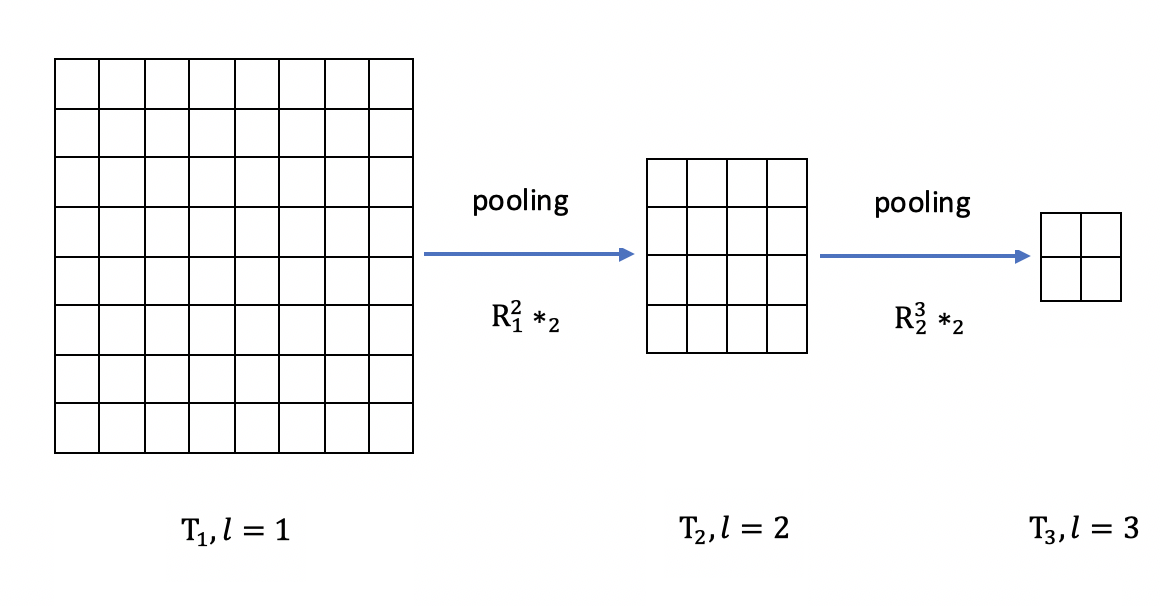
\includegraphics[width=.85\textwidth]{figures/multiresolution-CNN}
\end{figure}

Then we will introduce some classical architectures in convolution neural 
networks.


\subsection{LeNet-5, AlexNet and VGG}
LeNet-5 \cite{lecun1998gradient} is aconvolutional network designed for handwritten and machine-printed character recognition.  AlexNet \cite{krizhevsky2012imagenet} showed, for the first time, that the features obtained by learning can transcend manually-designed features, breaking the previous paradigm in computer vision. While previous derivatives of AlexNet focused on smaller window sizes and strides in the first convolutional layer, VGG \cite{simonyan2014very} addresses another very important aspect of CNNs: depth.

The  LeNet-5, AlexNet and VGG
can be written as:
\begin{breakablealgorithm}
	\footnotesize
	\caption{$ h = \text{Classic CNN}(f; J,\nu_1, \cdots, \nu_J)$}
	\label{alg:presnet}
	\begin{algorithmic}[1]
		\State Initialization:  $f^{1,0} = f_{\rm in}(f)$.
		%		\State Initialization $u^{1,0}$
		\For{$\ell = 1:J$}
		\For{$i = 1:\nu_\ell$}
		\State Basic Block:
		\begin{equation}\label{ori-ResNet}
		f^{\ell,i} = \sigma \left( \theta^{\ell,i} \ast f^{\ell,i-1}\right)
		\end{equation}
		\EndFor
		%		\State Note: $ u^\ell= u^{\ell,\nu_\ell} $
		\State Pooling(Restriction):
		\begin{equation}
		\label{ori-ResNet0}
		f^{\ell+1,0} = R_\ell^{\ell+1} \ast_2 f^{\ell, \nu_\ell} 
		\end{equation}
		\EndFor
		\State Final average pooling layer:
		$h =  R_{\rm ave}( f^{L,\nu_\ell})$.
	\end{algorithmic}
\end{breakablealgorithm}

Here $R_\ell^{\ell+1} \ast_2$ represents for the pooling operation to 
sub-sampling these tensors into coarse spatial level (lower resolution).
Here we use $R_\ell^{\ell+1} \ast_2$ to stand for the pooling operation. 
In general we can also have
\begin{itemize}
	\item average pooling: fixed kernels such as 
	\begin{equation}\label{key}
	R_\ell^{\ell+1}  = \frac{1}{9} 
	\begin{pmatrix}
	1 & 1 & 1 \\
	1 & 1 & 1 \\
	1 & 1 & 1
	\end{pmatrix}
	\end{equation}
	\item Max pooling $R_{\rm max}$ as discussed before.
\end{itemize}

In these classic CNN models, they still need some 
extra fully connected layers after $h$ as the output of CNNs. 
After few layers of fully connected layers, the model is completed by following
a multi-class logistic regression model.

These fully connected layers are removed in ResNet to be described below.


\subsection{ResNet}
The original ResNet developed in~\cite{he2016deep} is one
of the most popular CNN architectures in image classification problems.
\begin{breakablealgorithm}
	\footnotesize
	\caption{$ h = \text{ResNet}(f; J,\nu_1, \cdots, \nu_J)$}
	\label{alg:resnet}
	\begin{algorithmic}[1]
		\State Initialization:  $r^{1,0} = f_{\rm in}(f)$.
		%		\State Initialization $u^{1,0}$
		\For{$\ell = 1:J$}
		\For{$i = 1:\nu_\ell$}
		\State Basic Block:
		\begin{equation}\label{ori-ResNet}
			r^{\ell,i} = \sigma\left(r^{\ell, i-1} + A^{\ell,i} \ast  \sigma \circ B^{\ell,i}\ast r^{\ell,i-1}\right).
		\end{equation}
		\EndFor
		%		\State Note: $ u^\ell= u^{\ell,\nu_\ell} $
		\State Pooling(Restriction):
		\begin{equation}
			\label{ori-ResNet0}
			r^{\ell+1,0} = \sigma \left( R_\ell^{\ell+1} \ast_2  r^{\ell, \nu_\ell} + A^{\ell+1,0} \circ \sigma \circ B^{\ell+1,0} \ast_2 r^{\ell, \nu_\ell} \right).
		\end{equation}
		\EndFor
		\State Final average pooling layer:
		$h =  R_{\rm ave}( r^{L,\nu_\ell})$.
	\end{algorithmic}
\end{breakablealgorithm}
Here $f_{\rm in}(\cdot)$ may depend on different data set and problems 
such as $f_{\rm in}(f) = \sigma \circ \theta^0 \ast f $ for CIFAR~\cite{krizhevsky2009learning} and
$f_{\rm in}(f) = R_{\rm max}\circ \sigma \circ \theta^0 \ast  f$ for ImageNet~\cite{deng2009imagenet} as in~\cite{he2016identity}.
In addition $r^{\ell,i} =   r^{\ell, i-1} +  A^{\ell,i} \ast  \sigma \circ B^{\ell,i} \ast \sigma (r^{i-1})$ is often called the basic ResNet block.
Here, $A^{\ell,i}$ with $i\ge0$ and $B^{\ell,i}$ with $i\ge1$ are general $3\times3$ convolutions with zero padding and stride 1.
In pooling block, $\ast _2$ means convolution with stride 2 and $B^{\ell,0}$ is taken as the $3\times3$ kernel with same output channel dimension of $R_\ell^{\ell+1}$
which is taken as $1\times1$ kernel and called as projection operator in \cite{he2016identity}. 
During two consecutive pooling blocks, index $\ell$ means the fixed resolution or we $\ell$-th grid level as in multigrid methods.
Finally, $R_{\rm ave}$ ($R_{\rm max}$) means average (max) pooling with different strides which is also dependent on datasets and problems.


\subsection{pre-act ResNet} 
The pre-act ResNet~\cite{he2016identity} shares a similar
structure with ResNet. 
\begin{breakablealgorithm}
	\footnotesize
	\caption{$ h = \text{pre-act ResNet}(f; J,\nu_1, \cdots, \nu_J)$}
	\label{alg:presnet}
	\begin{algorithmic}[1]
		\State Initialization:  $r^{1,0} = f_{\rm in}(f)$.
		%		\State Initialization $u^{1,0}$
		\For{$\ell = 1:J$}
		\For{$i = 1:\nu_\ell$}
		\State Basic Block:
		\begin{equation}\label{ori-ResNet}
			r^{\ell,i} = r^{\ell, i-1} + A^{\ell,i} \ast  \sigma \circ B^{\ell,i}\ast   \sigma (r^{\ell,i-1}).
		\end{equation}
		\EndFor
		%		\State Note: $ u^\ell= u^{\ell,\nu_\ell} $
		\State Pooling(Restriction):
		\begin{equation}
			\label{ori-ResNet0}
			r^{\ell+1,0} = R_\ell^{\ell+1} \ast_2  r^{\ell, \nu_\ell} + A^{\ell+1,0} \circ \sigma \circ B^{\ell+1,0} \ast_2  \sigma (r^{\ell, \nu_\ell} ).
		\end{equation}
		\EndFor
		\State Final average pooling layer:
		$h =  R_{\rm ave}( r^{L,\nu_\ell})$.
	\end{algorithmic}
\end{breakablealgorithm}
Here pre-act ResNet share almost the same setup with ResNet.


The only difference between ResNet and pre-act ResNet can be viewed as 
putting a $\sigma$ in different places. 
The connection of those three models are often shown with next diagrams:
\begin{figure}[!htb]
	\begin{center}
		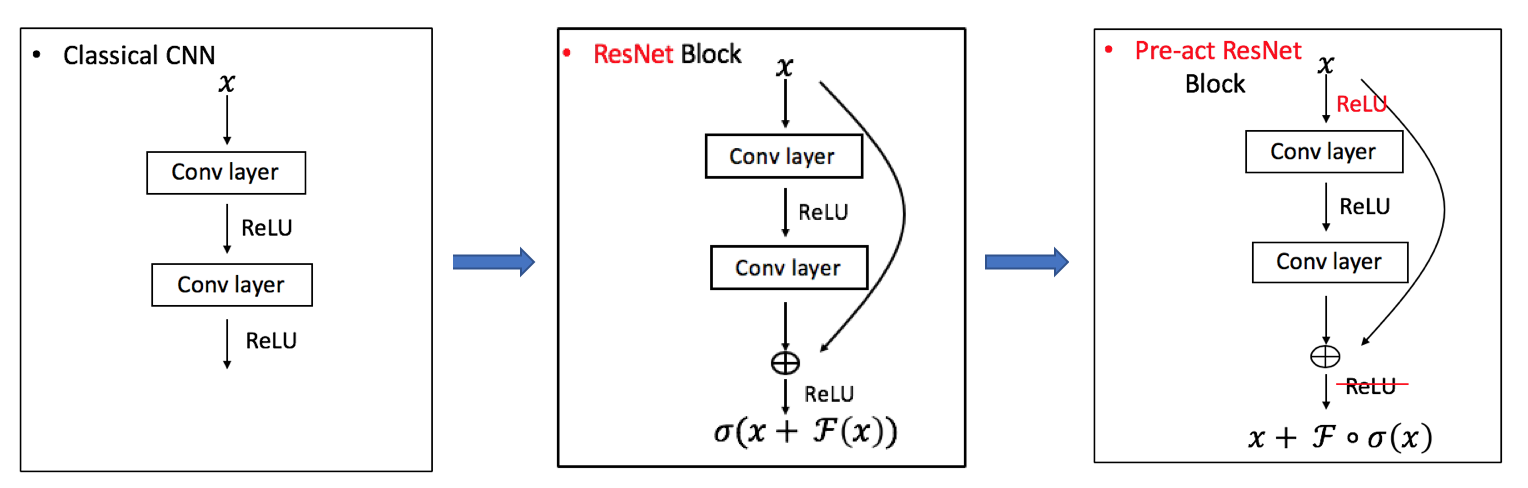
\includegraphics[width=.6\textwidth, height=.13\textheight]{CNN_ResNet} 
	\end{center}
	\caption{Comparison of CNN Structures}
\end{figure}

Without loss of generality, we extract the key 
feedforward steps on the same grid in different CNN models as follows.
\begin{description}
	\item[Classic CNN] 
	\begin{equation}\label{eq:cCNN}
	f^{\ell,i} = \xi^i \circ \sigma (f^{\ell,i-1}) \quad \text{or} \quad f^{\ell,i} = \sigma \circ \xi^{i} (f^{\ell,i-1}) .
	\end{equation}
	\item[ResNet] 
	\begin{equation}\label{eq:ResNet}
	r^{\ell,i} = \sigma( r^{\ell,i-1} + A^{\ell,i} \circ \sigma \circ B^{\ell,i}(r^{\ell,i-1})).
	\end{equation}
	\item[pre-act ResNet]
	\begin{equation}\label{eq:pre-act ResNet}
	r^{\ell,i} = r^{\ell,i-1} + A^{\ell,i} \circ \sigma \circ B^{\ell,i}\circ \sigma(r^{\ell,i-1}).
	\end{equation}
\end{description} 